%%%%%%%%%%%%%%%%%%%%%%%%%%  phdsymp_sample2e.tex %%%%%%%%%%%%%%%%%%%%%%%%%%%%%%
%% changes for phdsymp.cls marked with !PN
%% except all occ. of phdsymp.sty changed phdsymp.cls
%%%%%%%%%%                                                       %%%%%%%%%%%%%
%%%%%%%%%%    More information: see the header of phdsymp.cls   %%%%%%%%%%%%%
%%%%%%%%%%                                                       %%%%%%%%%%%%%
%%%%%%%%%%%%%%%%%%%%%%%%%%%%%%%%%%%%%%%%%%%%%%%%%%%%%%%%%%%%%%%%%%%%%%%%%%%%%%%


%\documentclass[10pt]{phdsymp} %!PN
\documentclass[twocolumn]{phdsymp} %!PN
%\documentclass[12pt,draft]{phdsymp} %!PN
%\documentstyle[twocolumn]{phdsymp}
%\documentstyle[12pt,twoside,draft]{phdsymp}
%\documentstyle[9pt,twocolumn,technote,twoside]{phdsymp}

\usepackage[english]{babel}       % Voor nederlandstalige hyphenatie (woordsplitsing)

\usepackage{graphicx}                   % Om figuren te kunnen verwerken
\usepackage{graphics}			% Om figuren te verwerken.
\graphicspath{{fig/}}               % De plaats waar latex zijn figuren gaat halen.

\usepackage{times}

\hyphenation{bij-gehouden privacy-vriendelijke analyse beoordeeld}

\def\BibTeX{{\rm B\kern-.05em{\sc i\kern-.025em b}\kern-.08em
    T\kern-.1667em\lower.7ex\hbox{E}\kern-.125emX}}

\newtheorem{theorem}{Theorem}

\begin{document}

\title{Een privacyvriendelijk aanbevelingssysteem\\ voor mobiele toestellen} %!PN

\author{Thorwald Frederik Lambrecht}

\supervisor{Marleen Denert, Luc Martens, Toon De Pessemier}

\maketitle

\begin{abstract}
Dit artikel probeert het ideale privacyvriendelijke aanbevelingssysteem te cre\"eren voor een mobiel toestel. In dit proces zal het trachten de grenzen van de wisselwerking tussen privacy, nauwkeurigheid en performantie bij aanbevelingssystemen te verleggen. Om dit te bereiken wordt een methode gebruikt op basis van homomorfische encryptie.
\end{abstract}

\begin{keywords}
Privacy, mobiel, aanbevelingssysteem
\end{keywords}

\section{Inleiding}
\PARstart{O}{m} gepersonaliseerde aanbevelingen toe te laten hebben aanbevelingssystemen privacygevoelige data nodig van hun gebruikers. Dit verplicht de \emph{service provider} om deze data bij te houden en 
opent de poort voor de privacy inbreuken. Deze inbreuken kunnen het gevolg zijn van een oneerlijke provider of een na\"ieve gebruiker, maar ook van onvoldoende data bescherming tegenover aanvallen van derden.\\ Er bestaan verschillende benaderingen om de privacy van de gebruiker te verbeteren. Eerst en vooral kan de gebruiker beter ingelicht worden over de grootteorde waarop zijn data wordt bijgehouden en de wijze waarop ze gebruikt wordt. Ten tweede zou de wet rond privacy strikter kunnen gemaakt worden. Een andere mogelijkheid is het gebruik van privacyvriendelijke algoritmes.\\
Het gebruik van bestaande algoritmes vermindert ofwel de nauwkeurigheid van de aanbevelingen ofwel de prestatie ofwel beide. Rekening houdend met de mobiele setting, is het ook belangrijk om een werkwijze te vinden die niet veel processortijd of data overdracht vraagt op de client. Om uit te zoeken hoe een aanbevelingssysteem in een mobiele setting de wisselwerking best aanpakt, was er onderzoek nodig naar de bestaande privacyvriendelijke oplossingen.

\section{Onderzoek naar bestaande privacyvriendelijke methodes}
Er bestaan verschillende methodes om de privacy te verbeteren in aanbevelingssystemen. Deze methodes omvatten werkwijzes met behulp van anonimisatie, randomisatie, aggregatie van gebruikersprofielen en cryptografische protocollen. Voor elk van deze mogelijkheden werd er een grondige analyse gemaakt van minstens \'e\'en voorbeeldoplossing. Daarna werd er een vergelijking gemaakt tussen de oplossingen onderling om te besluiten welke methode het best aansluit bij een mobiele setting. \\ De oplossing gebaseerd op anonimisatie \cite{anonimisatie} maakt gebruik van agents die anoniem communiceren met elkaar. Ondanks het feit dat gedurende de aanvragen en de vergelijking van gebruikers onderling voor user-user collaborative filtering, de gebruikers anoniem blijven, garandeert anonimiteit geen privacy. Dit is bewezen door Narayan \cite{anon}.\\ Het randomisatie algoritme gebruikt door Polat en Du \cite{rand} voorziet ook niet in volledige privacy voor de gebruiker, aangezien de server nog steeds de range van waarden weet waartussen een gebruiker zijn aparte waarden liggen. De methode verliest ook sterk aan nauwkeurigheid bij het gebruik van kleine datasets.\\  Het gebruik van aggregatie van gebruikersprofielen door Shokri et al. in \cite{agg} biedt de gebruiker de mogelijkheid om zijn voorkeuren te ontkennen maar toont de server nog steeds originele beoordelingen van de gebruiker. Deze werkwijze verliest boet wel niet aan nauwkeurigheid in. \\ De oplossing aan de hand van cryptografische protocollen met gebruik van een peer-to-peer relatie tussen clients \cite{social} is wel privacyvriendelijk maar heeft een sociaal netwerk nodig waar gebruikers vaak online zijn. De methode vraagt ook te veel berekeningen aan de clientkant voor een mobiele setting.\\ De beste methode lijkt deze op basis van cryptografische protocollen met twee servers door Erkin et al \cite{dyn}. Deze aanpak gebaseerd op een eerdere oplossing \cite{erkin} biedt een hoog privacyniveau en vereist geen zware berekeningen aan de clientkant. Op basis van deze vaststellingen werden de cryptografische protocollen van deze methode gekozen om te dienen als basis voor deze oplossing.

\section{De privacyvriendelijke oplossing}
We besloten om een native androidapplicatie te maken en de servers werden geschreven in Java. Ze communiceren allemaal onderling met het HTTP-protocol. Als testdatabank werd de MovieLens databank gebruikt met 100.000 beoordelingen, 943 personen en 1682 films. De oplossing in \cite{dyn} maakt gebruik van twee servers, een aanbevelingsserver en een tweede server die wordt ingezet door een betrouwbare derde partij. De clientapplicatie stuurt de beoordelingen en voorkeuren van de gebruikers naar de aanbevelingsserver, ze zijn ge\"encrypteerd met de publieke Pailliersleutel van de tweede server. Dit hoeft niet elke keer te gebeuren als een gebruiker een item beoordeelt. Om een voorspelling te doen van een beoordelingswaarde voor een item is er communicatie nodig tussen de twee servers op basis van hun Paillier en DGK cryptosysteem. Zo wordt in de originele paper het aantal en de som van de ge\"encrypteerde ratings van gebruikers met gelijkaardige voorkeuren geteld. Door deze te delen kan de client de gemiddelde rating van gelijkaardige gebruikers bepalen. De gelijkaardigheid tussen twee gebruikers wordt bepaald door de gekende Pearson-correlatie, die hier ook deels door de client wordt berekend. Om de berekeningen van de Pearsoncorrelatie aan de serverkant te maken worden ingewikkelde protocollen zoals een vermenigvuldigingsprotocol en een drempelprotocol gebruikt. \\Er zijn verschillende praktische beslissingen die moeten genomen worden tijdens het implementeren van deze protocollen, vooral aan de clientkant: In tegenstelling tot \cite{dyn} zou de gebruiker zijn ge\"encrypteerde waarden best niet stuk per stuk opsturen als hij een item beoordeelt. Dit zou aan de service provider laten weten welke items de persoon geratet heeft. Een mogelijkheid is om een aantal willekeurige items te kiezen en de beoordelingen hiervan mee te sturen. Indien deze items niet beoordeeld zijn wordt een nulwaarde ge\"encrypteerd en meegestuurd. Toch kan hiermee nog privacy lekken indien alle random gekozen items dezelfde eigenschappen hebben. Dit kan worden vermeden door deze items op een slimme manier te kiezen, maar dit laat wel zijn offsets (zie later) en voorkeuren berekend op een oude versie van het gemiddelde. Om optimale privacy in onze applicatie te bereiken stuurt de gebruiker zijn ratings en voorkeuren, samen ook zijn profiel genoemd, in \'e\'en  keer naar de server. Hier berekent hij voor alle items zonder ratings een ge\"encrypteerde nulwaarde die hij meegeeft met zijn profiel.\\ Voor deze oplossing is het ook nodig dat per rating uit een profiel, een extra ge\"encrypteerde bit wordt meegegeven. Deze ge\"encrypteerde bit $ q_{U_x,i} $ is \"e\"en als de gebruiker x item i heeft beoordeeld en nul indien niet. Dit maakt het mogelijk om het aantal effectief ingevulde gebruikte ratings te bepalen in formule (\ref{stdrecom}). De encryptie van de beoordelingen wordt ook best berekend op het moment dat de gebruiker zijn profiel stuurt. Indien dit gebeurt onmiddelijk na een beoordeling en het hele profiel wordt opgestuurd kan, over tijd, de aanbevelingsserver vergelijken welke ge\"encrypteerde waarden veranderd zijn. In het origineel artikel \cite{dyn} wordt een voorspellingswaarde van een rating berekend door het gemiddelde te nemen van de beoordelingen van mensen met een gelijkaardigheidsscore boven een bepaalde drempelwaarde. Toch laten de protocollen een verbetering in deze wijze toe door voorspellingswaarden te genereren gebaseerd op een aangepaste versie van een formule die vaak wordt gebruikt in het user-user collaborative filtering:

\begin{equation}\label{stdrecom}p_{U_1,i} = \bar{r}_{U_1} + \frac{\sum_{j=2}^{n}(r_{(U_j,i)} - \bar{r}_{U_j}).s_{(U_1,U_j)}.q_{(U_j,i)}}{\sum_{j=2}^{n} s_{(U_1,U_j)}.q_{(U_j,i)} }
\end{equation}

Hier staat $r_{(U_x,i)}$ voor de beoordelingswaarde van user x voor item i, $\bar{r}_{U_x}$ de gemiddelde beoordelingswaarde van een gebruiker over alle items heen en $p_{U_x,i}$ voor de voorspellingswaarde voor gebruiker x, item i.
De waarde $s_{(U_1,U_j)}$ staat voor het bit dat is berekend door het drempelprotocol en het is 1 als de gebruiker een gelijkheidswaarde heeft boven de drempelwaarde. In de plaats van de beoordeling zelf zoals in \cite{dyn} wordt deze keer het verschil van de beoordeelde waarde $r_{(U_j,i)}$ en de gemiddelde waarde $\bar{r}_{U_1}$ van de gebruiker gestuurd. Deze waarde moet geconverteerd worden naar een positieve integer voor het gebruik van de cryptosystemen. Dit kan op een makkelijke manier gebeuren $result = ((r_{(U_j,i)} - \bar{r}_{U_j})+5)*1000$. Eenmaal de som is genomen over alle gelijkaardige gebruikers, kan de client de conversie omkeren door te delen met 1000 en dan 5 af te trekken per gelijkaardige gebruiker.


\section{Resultaten}

De voorspellingswaarden van de verbeterde methode (lichte lijn) tonen signifant betere scores op nauwkeurigheid dan de methode uit \cite{dyn} (de donkere lijn).

\begin{figure}[ht]
\begin{center}
	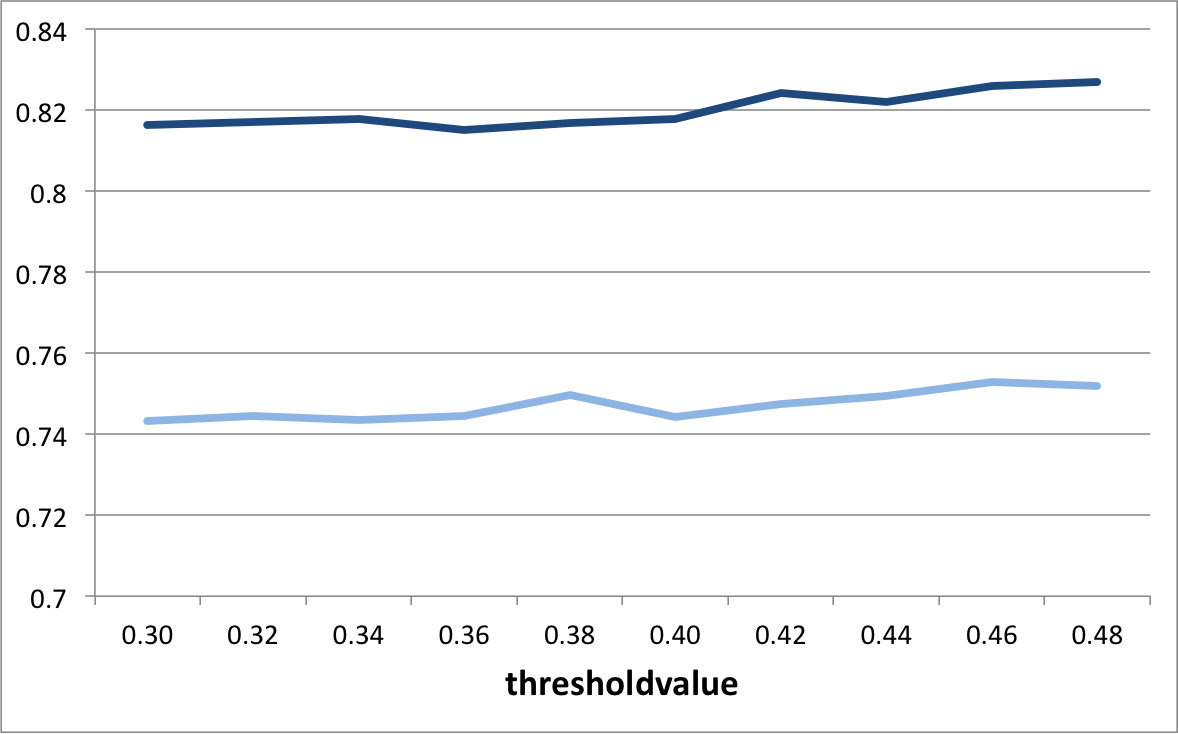
\includegraphics[width=.40\textwidth]{mae}
	\caption{MAE resultaten over 10.000 predictions berekend op verschillende drempelwaarden.}
\end{center}
\end{figure}
\begin{figure}[ht]
\begin{center}
	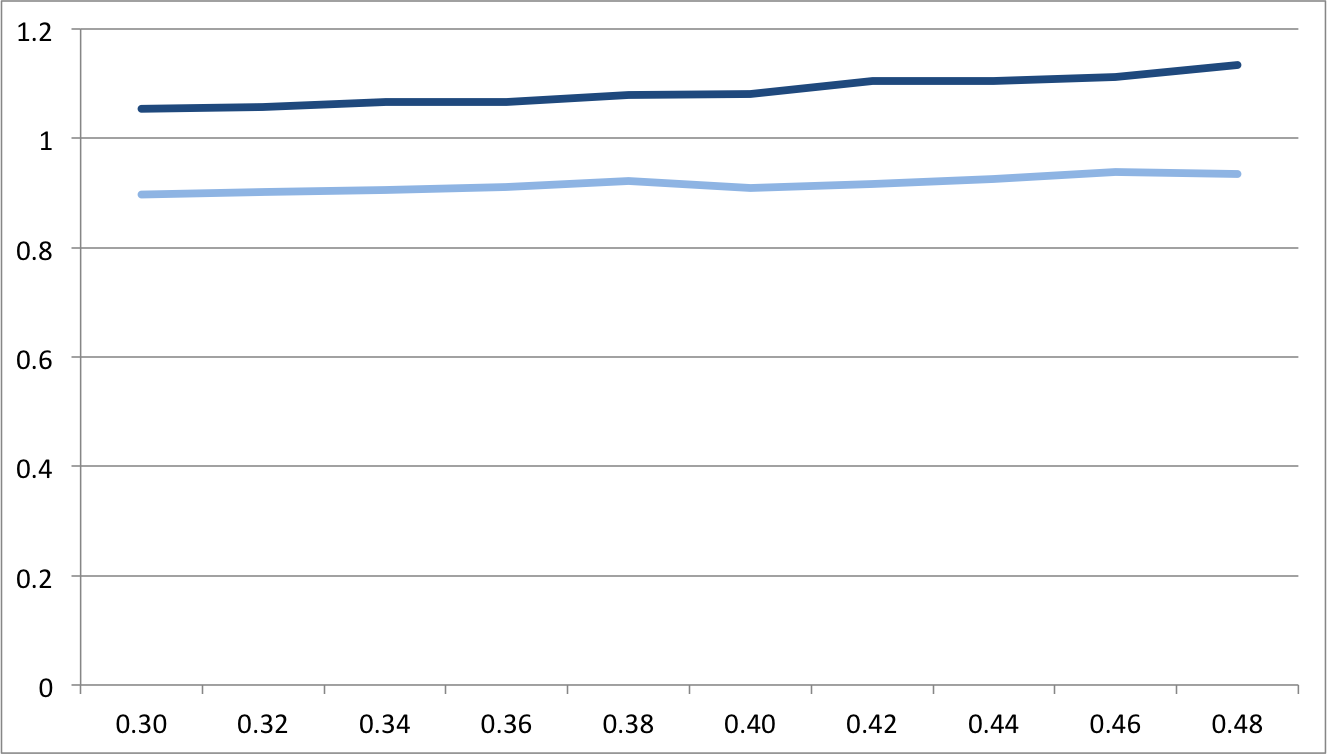
\includegraphics[width=.40\textwidth]{mse}
	\caption{MSE resultaten over 10.000 predictions berekend op verschillende drempelwaarden.}
\end{center}
\end{figure}

De MAE verbeterde van rond 0.82 ster to ongeveer 0.74 ster, dit is zeer dicht bij de MAE 0.7146 van de privacy-onvriendelijke oplossing op identiek dezelfde database door \cite{rand}. Sinds de privacy nog verbeterd is ten opzichte van de originele methode behaalt het een zeer hoog privacyniveau. 
Het uploaden van het profiel aan de clientkant is $O(N+S)$ met N als het aantal items en S als het aantal voorkeuren. Voor elk item gebeuren er 2 encrypties en voor elke voorkeur 1 encryptie. Deze encryptie gebeurde op het testtablet \footnote{Samsung Galaxy Tab4 (7.0) Wi-Fi on Android 4.4.2} in 1,52 seconden gemiddeld over 10 keer. De servers verrichten zware berekeningen, de testserver\footnote{MacBook Pro 4 GB RAM 2.4 GHZ i7 processor} had 7 minuten 26 seconden nodig om voorspellingswaarden te genereren voor alle 1682 items voor één gebruiker, als er gebruik wordt gemaakt van 30 preferences. Deze berekeningen kunnen echter nog geoptimaliseerd woord met het gebruik van een protocol op een lager niveau, want het was niet de beste keuze om het HTTP-protocol te gebruiken voor de communicatie tussen de twee servers. Ook is er een mogelijkheid om de gebruiker minder waarden naar de server te laten sturen zoals besproken. Dit zou een impact hebben op de nauwkeurigheid van het algoritme maar zou het werk aan de kant van de servers verminderen en de grootte van de database op de aanbevelingsserver beperken.
 
\section{Conclusion}

Deze oplossing garandeert een zeer hoog niveau van privacy door het gebruik van Paillier en DGK encryptie en het feit dat de server niet weer welke items beoordeeld zijn door de gebruiker. Hoge nauwkeurigheid wordt ook behaald zonder al te veel berekeningen aan de clientkant. Deze eigenschappen maken deze methode ideaal voor het gebruik als aanbevelingssysteem voor mobiele toestellen. De servers zelf doen zware berekeningen maar deze kunnen nog verder geoptimaliseerd worden.








\nocite{*}
\bibliographystyle{phdsymp}
%%%%%\bibliography{bib-file}  % commented if *.bbl file included, as
%%%%%see below


%%%%%%%%%%%%%%%%% BIBLIOGRAPHY IN THE LaTeX file !!!!! %%%%%%%%%%%%%%%%%%%%%%%%
%% This is nothing else than the phdsymp_sample2e.bbl file that you would%%
%% obtain with BibTeX: you do not need to send around the *.bbl file        
%%
%%---------------------------------------------------------------------------%%
%
\begin{thebibliography}{1}
\bibitem{anonimisatie}

Ciss{\'e}e, Richard and Albayrak, Sahin
\newblock {\em An Agent-based Approach for Privacy-preserving Recommender Systems},
\newblock Proceedings of the 6th International Joint Conference on Autonomous Agents and Multiagent Systems,2007

\bibitem{anon}
Narayanan, Arvind and Shmatikov, Vitaly
\newblock{\em Robust De-anonymization of Large Sparse Datasets},
\newblock Proceedings of the 2008 IEEE Symposium on Security and Privacy, 2008

\bibitem{rand}
Polat, Huseyin and Du, Wenliang
\newblock{\em SVD-based Collaborative Filtering with Privacy},
\newblock Proceedings of the 2005 ACM Symposium on Applied Computing,2005


\bibitem{agg}
Shokri, Reza and Pedarsani, Pedram and Theodorakopoulos, George and Hubaux, Jean-Pierre
\newblock{\em Preserving {P}rivacy in {C}ollaborative {F}iltering
                 through {D}istributed {A}ggregation of {O}ffline
                 {P}rofiles},
\newblock{The 3rd {ACM} {C}onference on {R}ecommender {S}ystems ({R}ec{S}ys), 2009}

\bibitem{dyn}
Zekeriya Erkin and Thijs Veugen and R.L. Lagendijk
\newblock{\em Privacy-Preserving Recommender Systems in Dynamic Environments},
\newblock IEEE Workshop on Information Forensics and Security, 2013

\bibitem{erkin}
Zekeriya Erkin and Michael Beye and Thijs Veugen and Reginald L. Lagendijk
\newblock{\em Efficiently computing private recommendations},
\newblock ICASSP,2011


\bibitem{social}
Hoens, T. Ryan and Blanton, Marina and Chawla, Nitesh V.
\newblock{\em A Private and Reliable Recommendation System for Social Networks},
\newblock{Proceedings of the 2010 IEEE Second International Conference on Social Computing, 2010}

\end{thebibliography}
%
%%---------------------------------------------------------------------------%%

\end{document}

%%%%%%%%%%%%%%%%%%%%%  End of phdsymp_sample2e.tex  %%%%%%%%%%%%%%%%%%%%%%%%%%%
